


\begin{figure}[t]%h!
    \centering
    \begin{subfigure}{.47\textwidth}
        \centering
        %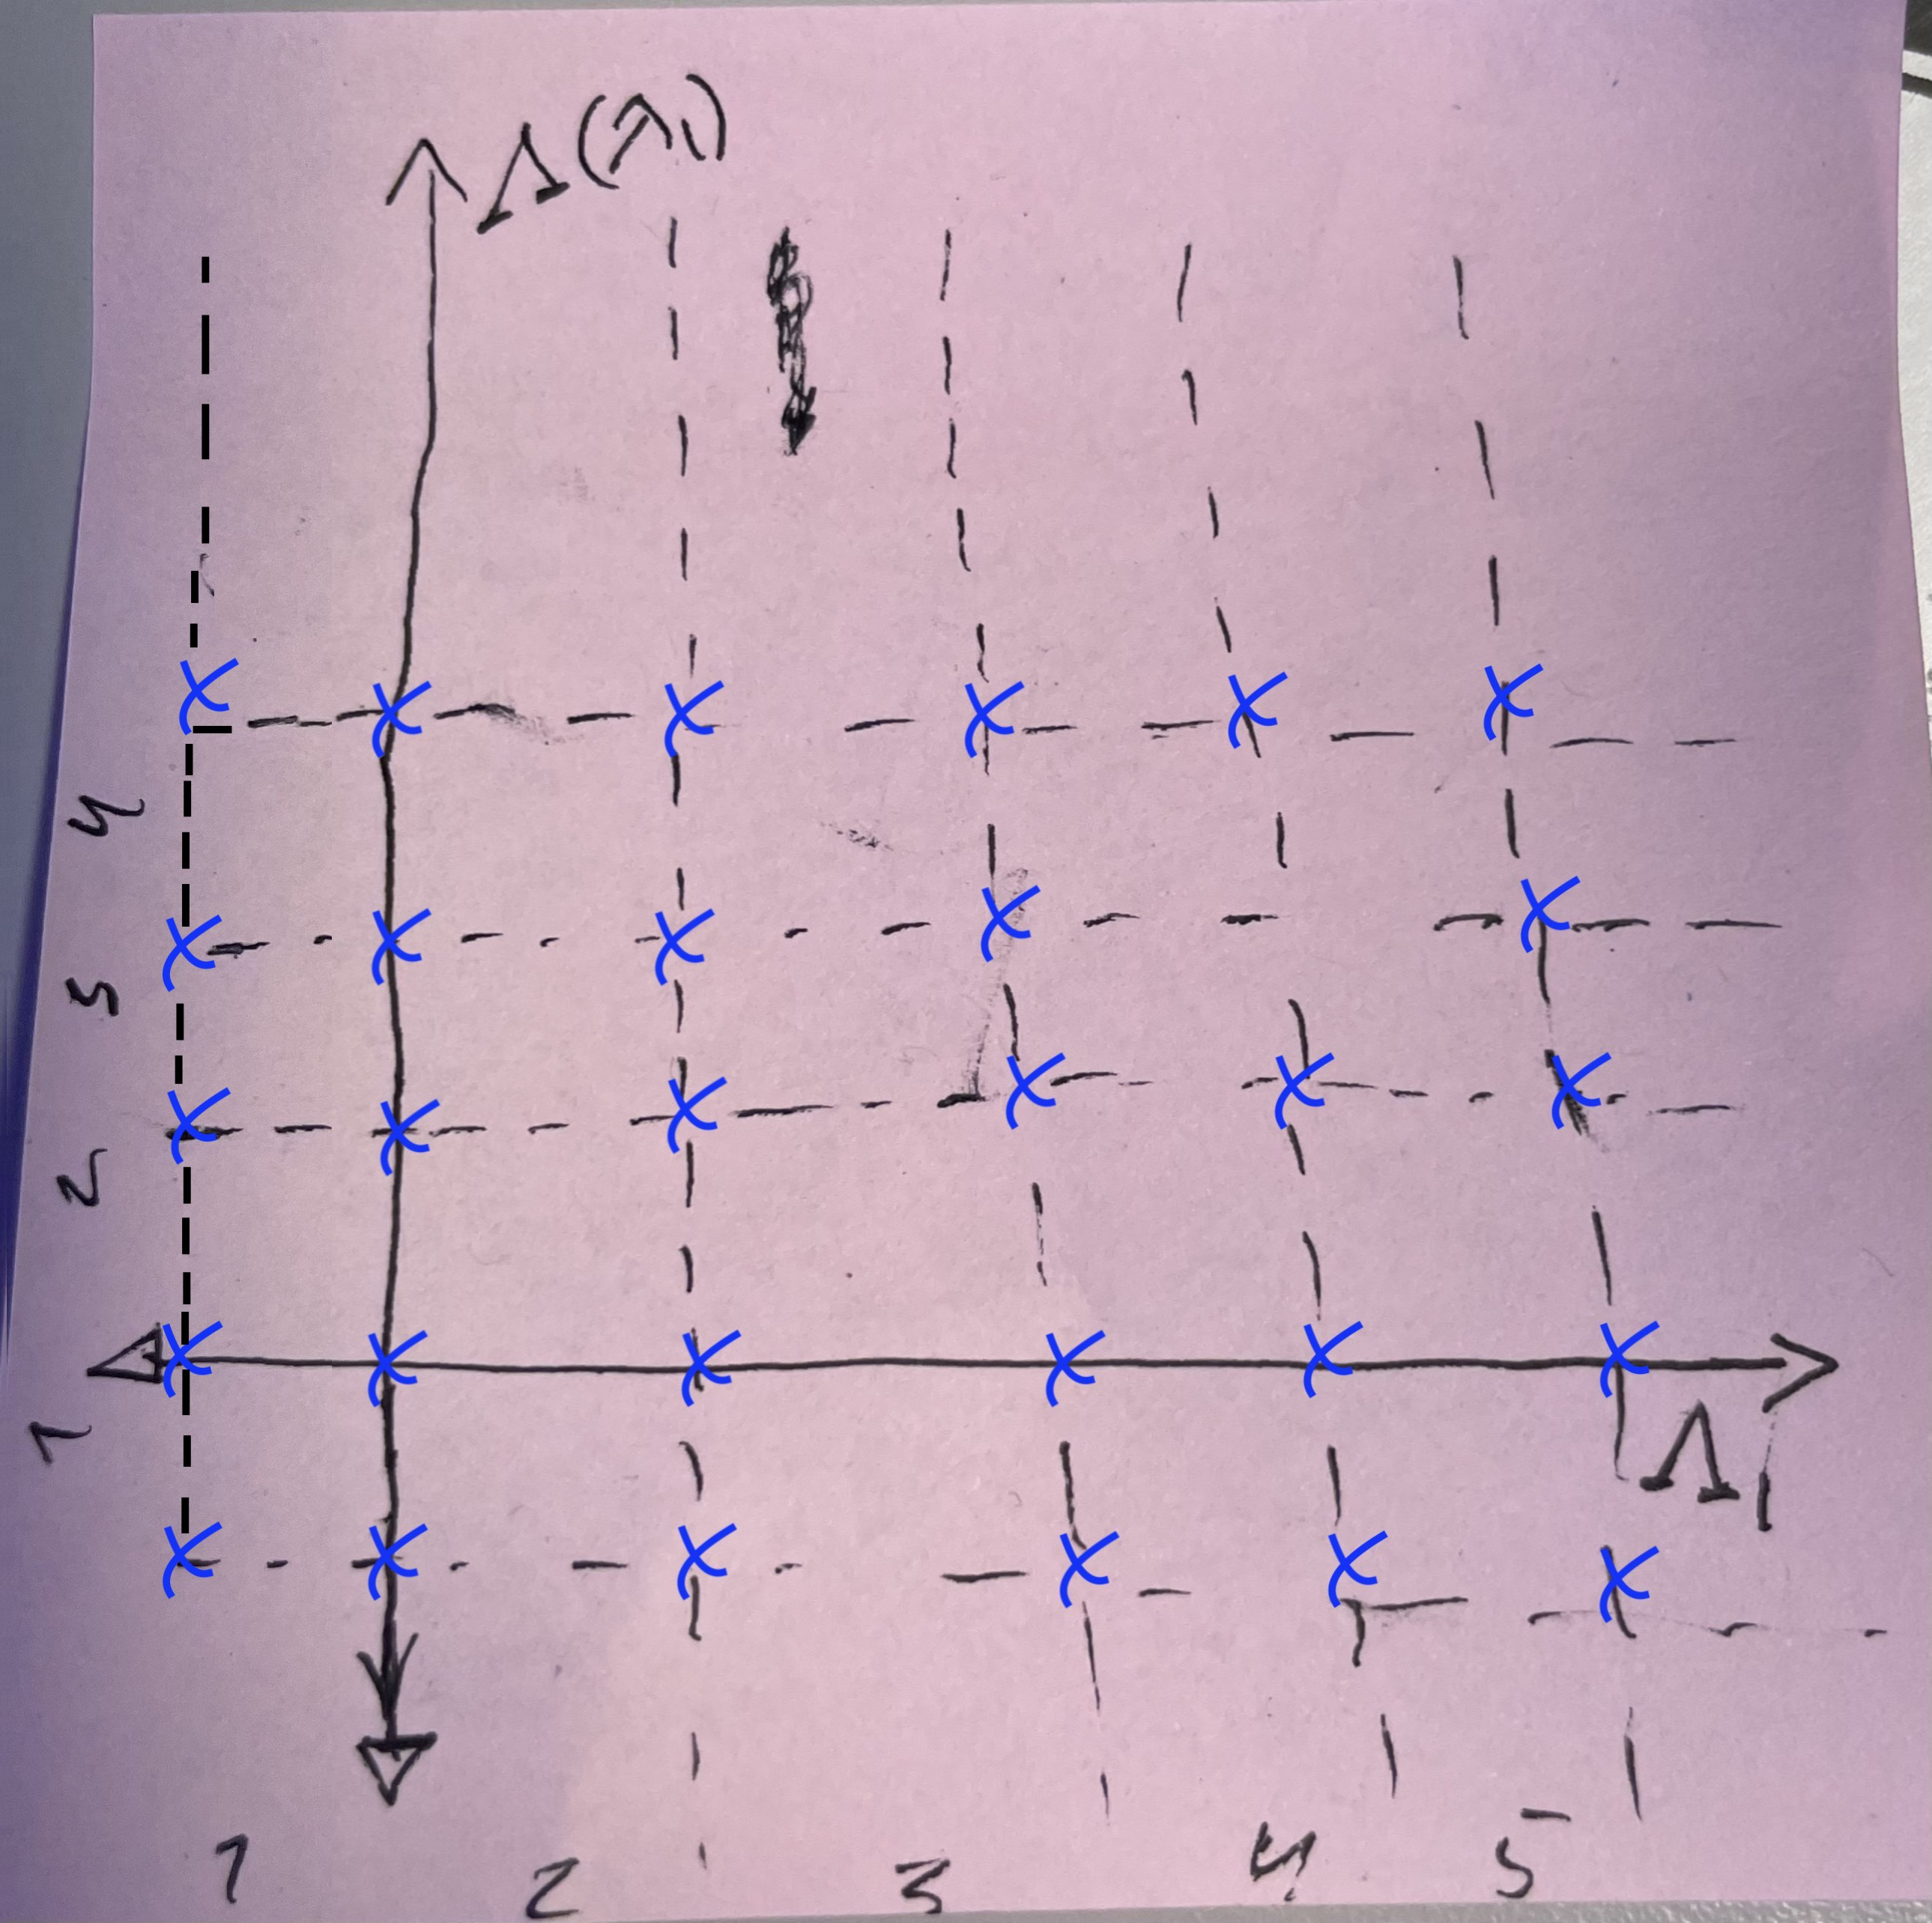
\includegraphics[width=0.9\linewidth]{spec_no_shift.jpg}
        %* Figure 1
        \begin{tikzpicture}[scale=1]
            % Define the tile
            \def\tile{
            \draw[fill=white] (0,0) rectangle (1,1);
            }
            \def\tiletwo{
            %\draw[black, fill=gray!65] (0,0) rectangle (1,1);
            %\draw[black, fill=cyan!65] (0,0) rectangle (1,1);
            \draw[pattern=north east lines, pattern color=MaxCyan] (0,0) rectangle (1,1);
            }
            
            % Draw the tiling pattern
            % Shifted line, part 1, left and right half tiles 
            \foreach \x in {0}{
                %\draw[cyan, fill=cyan] (\x-0.2,2) rectangle (\x+0.5,3);  % leftmost value to the first square
                \draw[white, pattern=north east lines, pattern color=MaxCyan] (\x-0.2,2) rectangle (\x+0.5,3); % leftmost value to the first square
            }
            \foreach \x in {6}{
                \draw[white, pattern=north east lines, pattern color=MaxCyan] (\x+0.2,2) rectangle (\x-0.5,3);
                %\draw[gray!65, fill=cyan!65] (\x+0.2,2) rectangle (\x-0.5,3);  % rightmost value to the last square
            }
            % part 2, whole tiles in the middle
            % must be after the above code in order to get black lines at the correct spots
            \foreach \y in {2}{
                \foreach \x in {0,1,2,3,4}{
                    \pgfmathsetmacro{\shiftX}{\x+0.5} % Set horizontal shift
                    \pgfmathsetmacro{\shiftY}{\y}
                    \begin{scope}[shift={(\shiftX,\shiftY)}]
                        \tiletwo
                    \end{scope}
                }
            }
            % Everything else
            \foreach \y in {0,1,3,4}{
                \foreach \x in {0,1,2,3,4,5}{
                    \pgfmathsetmacro{\shiftX}{\x} % Set horizontal shift
                    \pgfmathsetmacro{\shiftY}{\y}
                    \begin{scope}[shift={(\shiftX,\shiftY)}]
                        \tile
                    \end{scope}
                }
            }
            % get the outline grid 
            



% small black lines at the left and right
\foreach \y in {0,1,2,3,4,5}{
    \draw (0-0.2,\y) -- (0,\y);  % Left
    \draw (6,\y) -- (6+0.2,\y);  % Right
    
}

% small black lines at the top and bottom
\foreach \x in {0,1,2,3,4,5,6}{
    \draw (\x,0-0.2) -- (\x,0);  % Top
    \draw (\x,5) -- (\x,5+0.2);  % Bottom
}
        \end{tikzpicture}
        %* —————————————————
        \caption{Single row shift}
        \label{fig:single_shift_horizontal_tiling}
    \end{subfigure}\quad
    \begin{subfigure}{.47\textwidth}
        \centering
        %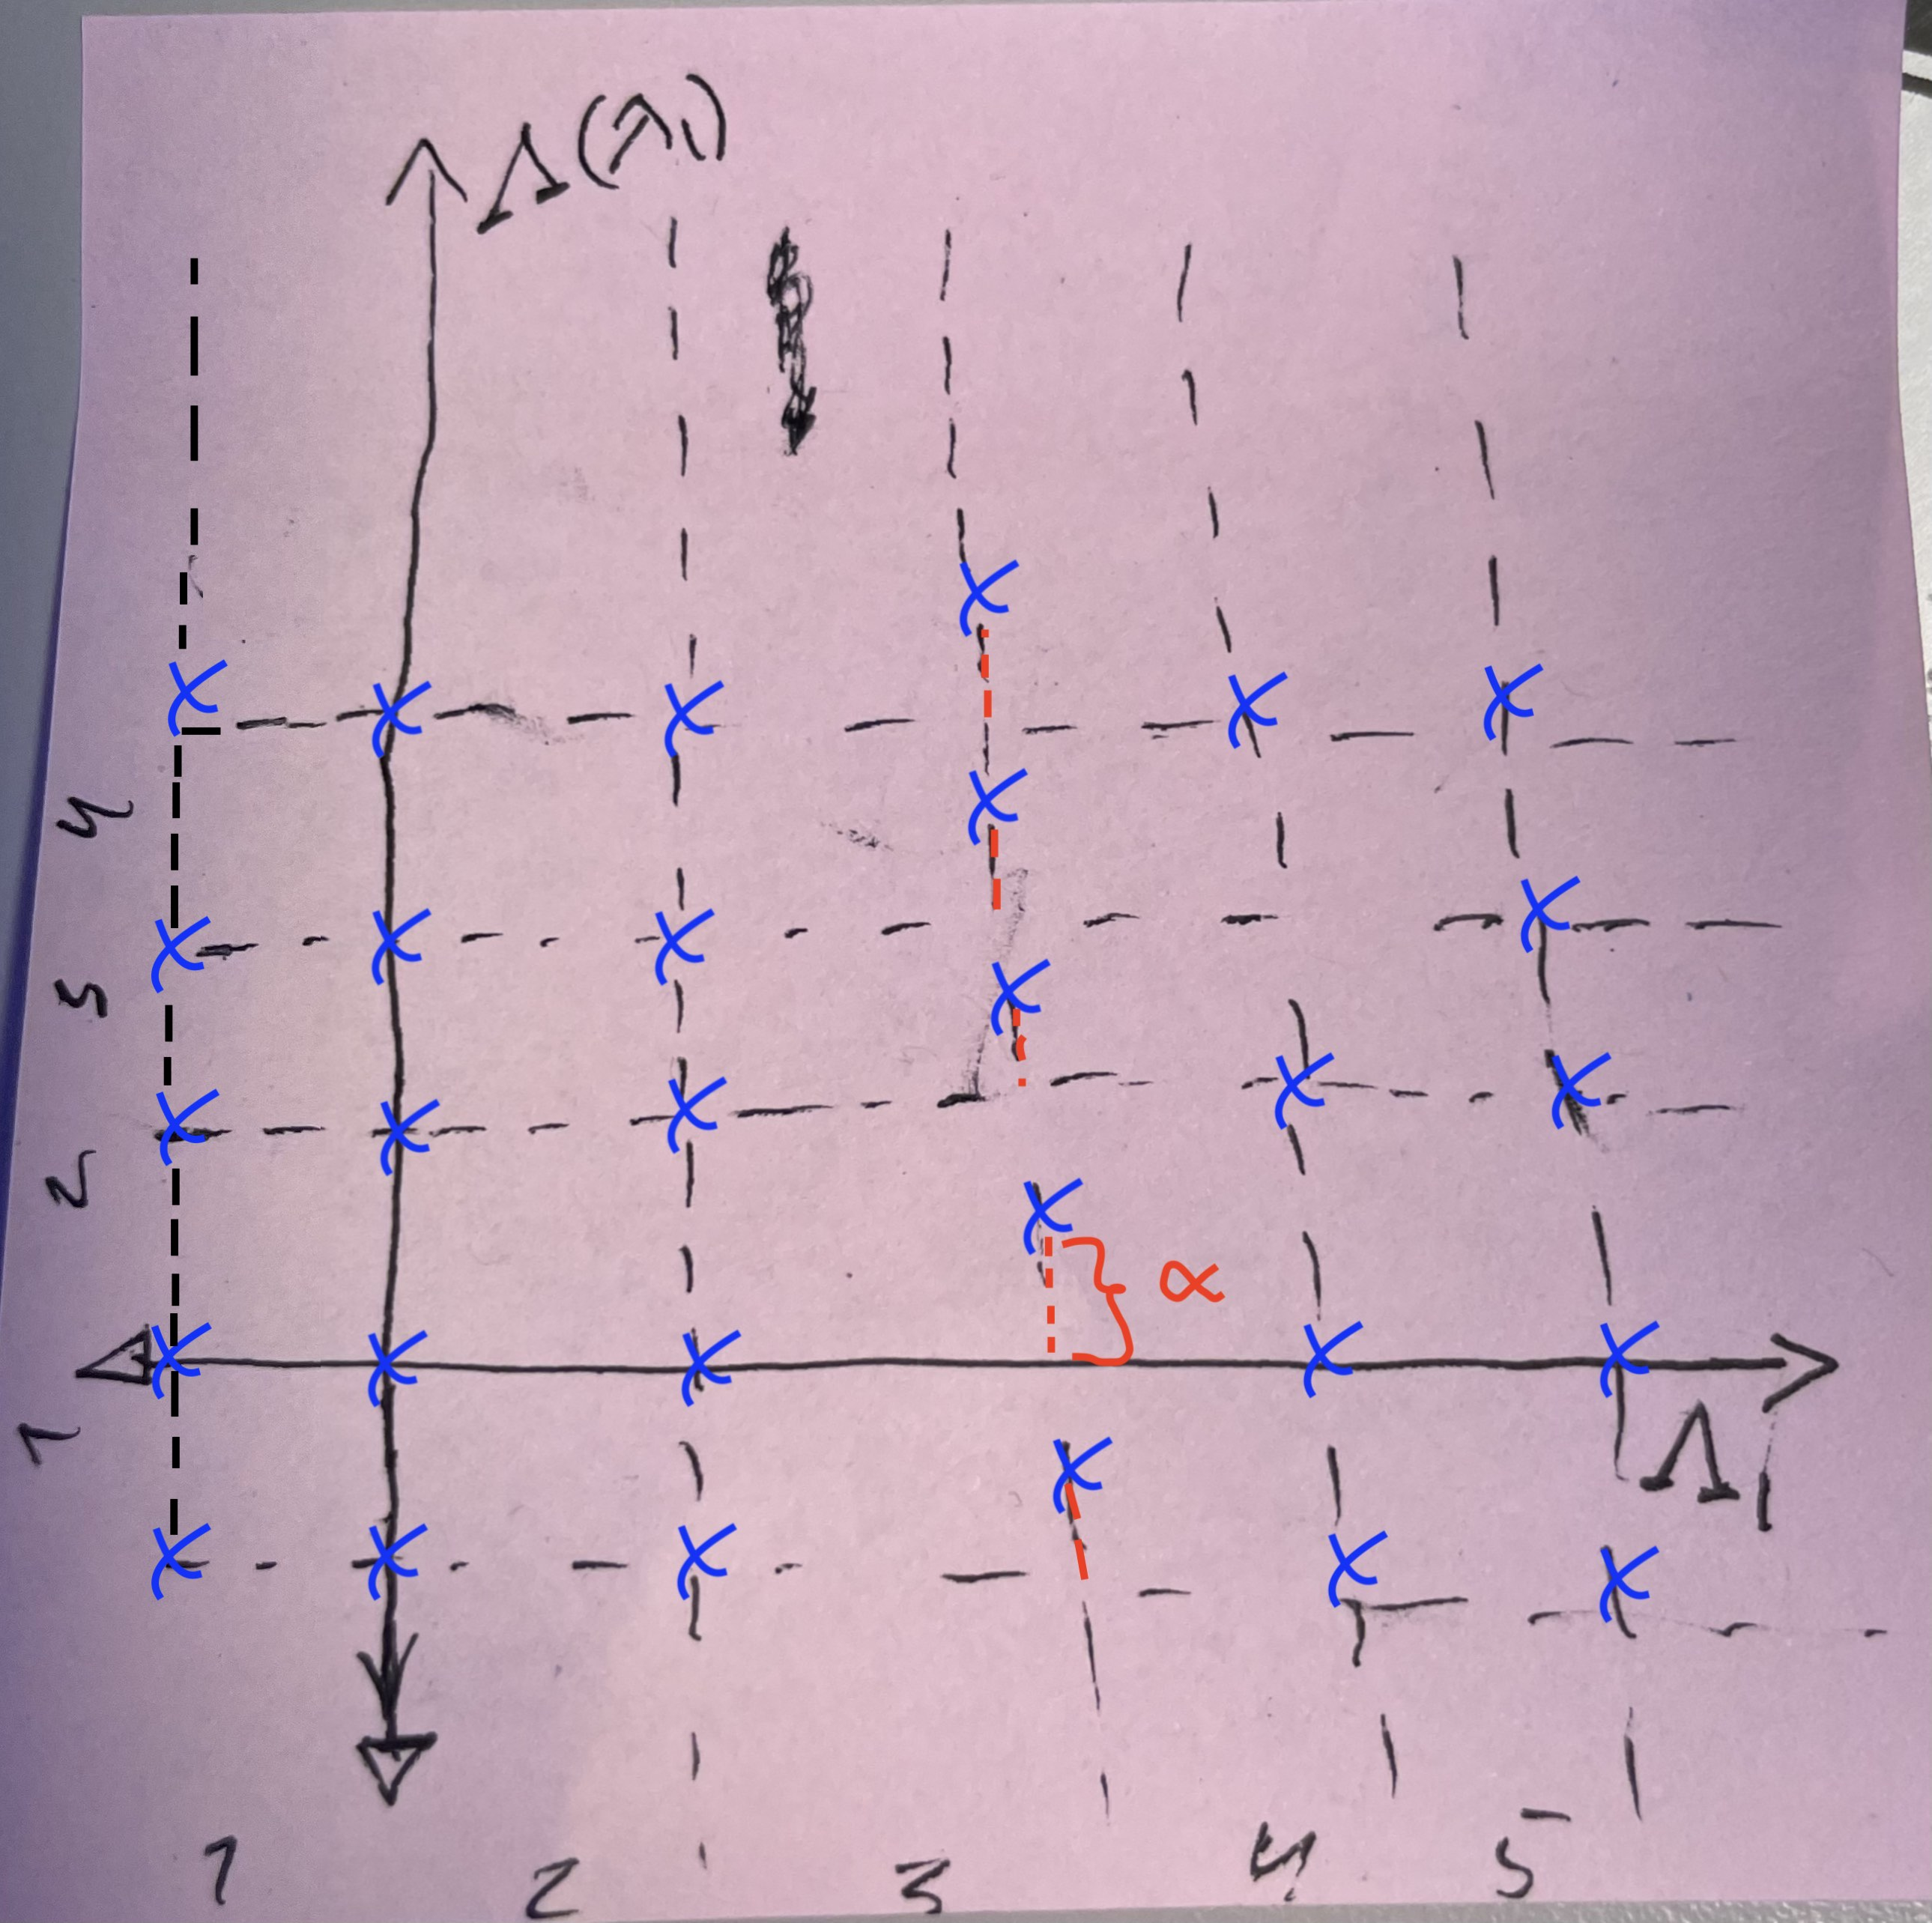
\includegraphics[width=0.9\linewidth]{spec_single_shift.jpg}
        %* Figure 2
        \begin{tikzpicture}[scale=1]
            % Define the tile
            \def\tile{
            \draw[fill=white] (0,0) rectangle (1,1);
            }
            \def\tiletwo{
            %\draw[fill=gray!65] (0,0) rectangle (1,1);
            %\draw[fill=YellowOrange] (0,0) rectangle (1,1);
            \draw[pattern=north east lines, pattern color=MaxOrange] (0,0) rectangle (1,1);
            }
            
            % Draw the tiling pattern
            % Shifted line, part 1, left and right half tiles 
            \foreach \y in {0}{
                %\draw[YellowOrange, fill=YellowOrange] (2,\y-0.2) rectangle (3,\y+0.5);
                \draw[white, pattern=north east lines, pattern color=MaxOrange] (2,\y-0.2) rectangle (3,\y+0.5);
                %\draw[orange!75, fill=orange!75] (2,\y-0.2) rectangle (3,\y+0.5);
            }
            \foreach \y in {5}{
                %\draw[YellowOrange, fill=YellowOrange] (2,\y+0.2) rectangle (3,\y-0.5);
                \draw[white, pattern=north east lines, pattern color=MaxOrange] (2,\y+0.2) rectangle (3,\y-0.5);
                %\draw[gray!65, fill=orange] (2,\y+0.2) rectangle (3,\y-0.5);
            }
            % part 2, whole tiles in the middle
            % must be after the above code in order to get black lines at the correct spots
            \foreach \x in {2}{
                \foreach \y in {0,1,2,3}{
                    \pgfmathsetmacro{\shiftX}{\x} % Set horizontal shift
                    \pgfmathsetmacro{\shiftY}{\y+0.5}
                    \begin{scope}[shift={(\shiftX,\shiftY)}]
                        \tiletwo
                    \end{scope}
                }
            }
            % Everything else
            \foreach \x in {0,1,3,4,5}{
                \foreach \y in {0,1,2,3,4}{
                    \pgfmathsetmacro{\shiftX}{\x} % Set horizontal shift
                    \pgfmathsetmacro{\shiftY}{\y}
                    \begin{scope}[shift={(\shiftX,\shiftY)}]
                        \tile
                    \end{scope}
                }
            }
            % get the outline grid 
            



% small black lines at the left and right
\foreach \y in {0,1,2,3,4,5}{
    \draw (0-0.2,\y) -- (0,\y);  % Left
    \draw (6,\y) -- (6+0.2,\y);  % Right
    
}

% small black lines at the top and bottom
\foreach \x in {0,1,2,3,4,5,6}{
    \draw (\x,0-0.2) -- (\x,0);  % Top
    \draw (\x,5) -- (\x,5+0.2);  % Bottom
}
        \end{tikzpicture}
        %* —————————————————
        \caption{Single column shift}
        \label{fig:single_shift_vertical_tiling}
    \end{subfigure}\\
    \begin{subfigure}{.47\textwidth}
        \centering
        %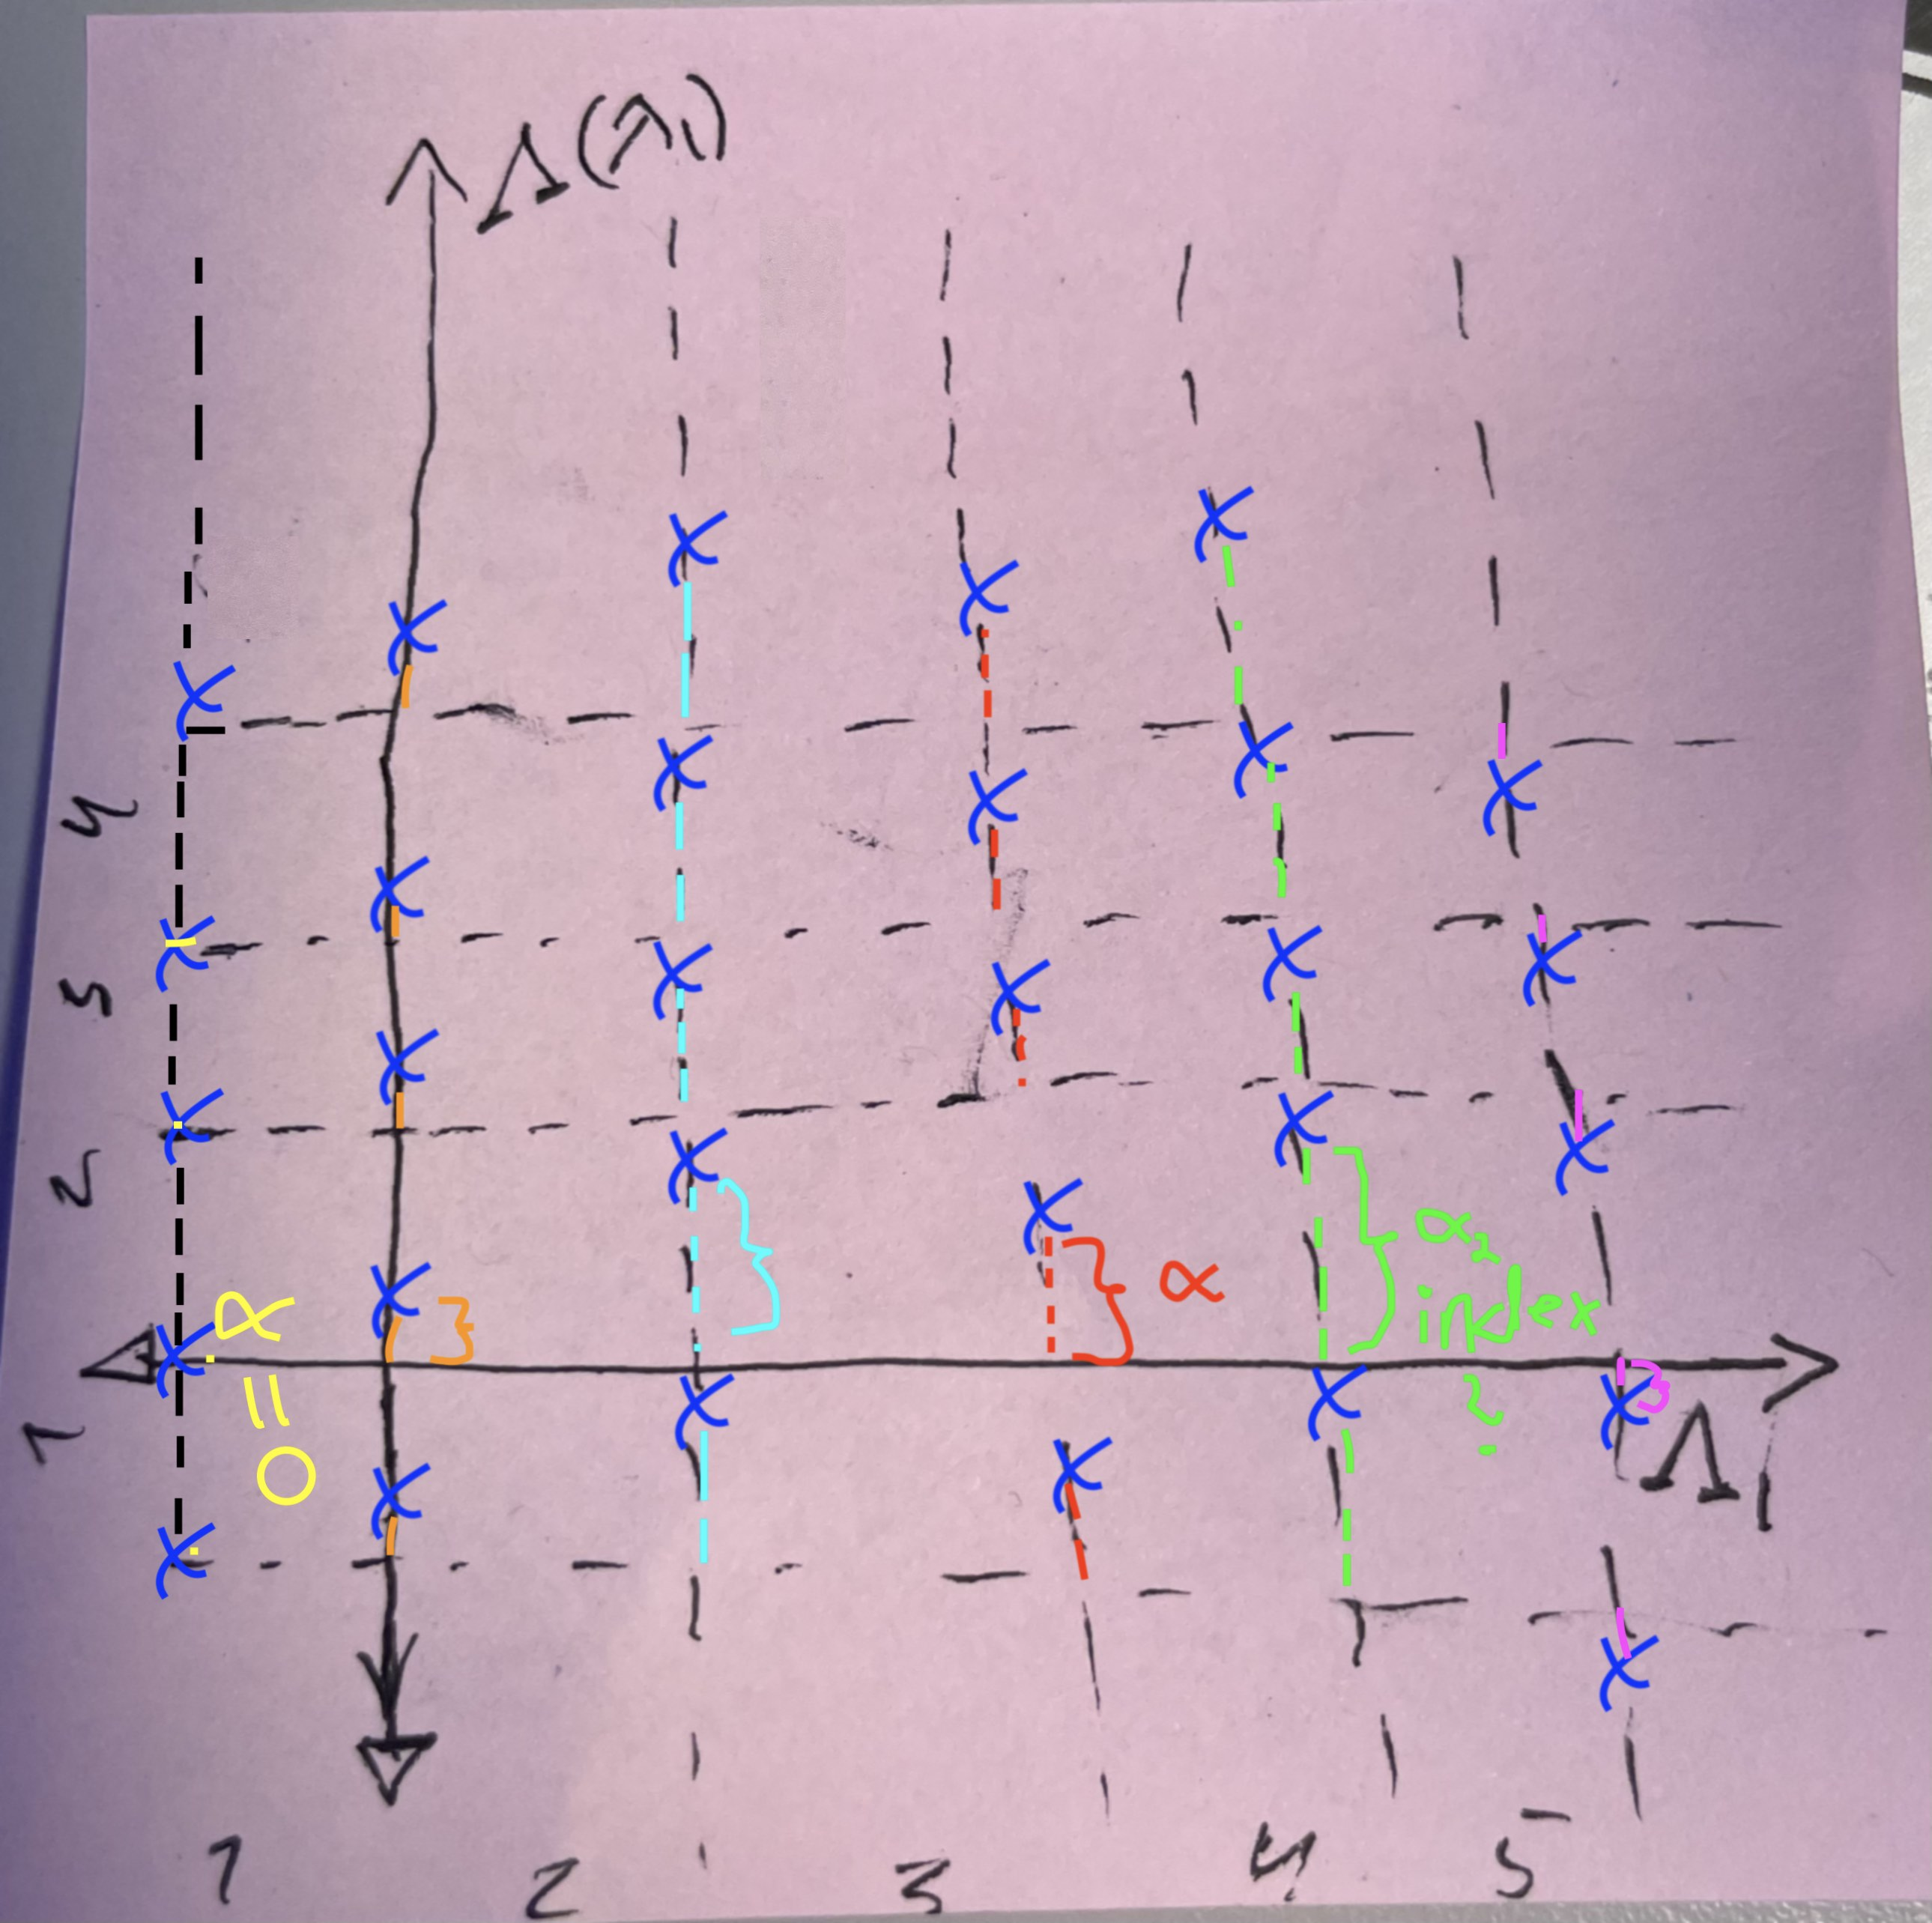
\includegraphics[width=0.9\linewidth]{multiple_shift_left_zero.jpg}
        %* Figure 3
        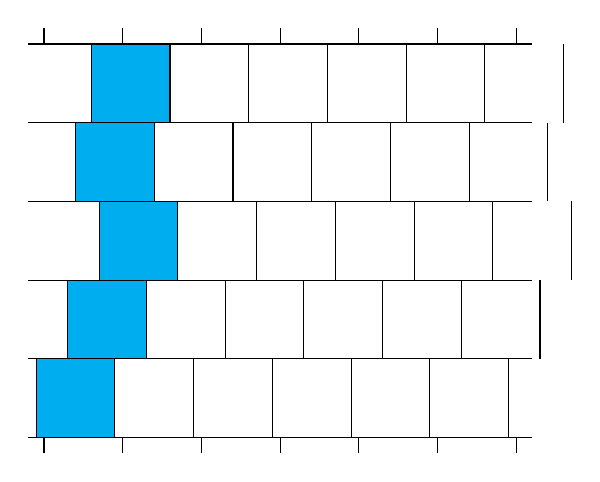
\begin{tikzpicture}[scale=1]
            % Define the tile
            \def\tile{
            % Draw the unit square
            \draw[fill=white] (0,0) rectangle (1,1);
            }
            \def\tiletwo{
            %\draw[fill=gray!65] (0,0) rectangle (1,1);
            \draw[fill=cyan] (0,0) rectangle (1,1);
            }

            % Shift list
            \def\BetaMinOne{-0.1}
            \def\BetaZero{0.3}
            \def\BetaOne{0.7}
            \def\BetaTwo{0.4}
            \def\BetaThree{0.6}
            
            % Draw the tiling pattern
            \foreach \x in {0,1,2,3,4}{
                \foreach \y in {0,1,2,3,4}{
                    \ifnum\y=0
                        \pgfmathsetmacro{\shiftX}{\x + \BetaMinOne}
                        \pgfmathsetmacro{\shiftY}{\y}
                        \pgfmathsetmacro{\shiftSingle}{\BetaMinOne}
                    \fi
                    \ifnum\y=1
                        \pgfmathsetmacro{\shiftX}{\x + \BetaZero}
                        \pgfmathsetmacro{\shiftY}{\y}
                        \pgfmathsetmacro{\shiftSingle}{\BetaZero}
                    \fi
                    \ifnum\y=2
                        \pgfmathsetmacro{\shiftX}{\x + \BetaOne} 
                        \pgfmathsetmacro{\shiftY}{\y} 
                        \pgfmathsetmacro{\shiftSingle}{\BetaOne}
                    \fi
                    \ifnum\y=3
                        \pgfmathsetmacro{\shiftX}{\x + \BetaTwo}
                        \pgfmathsetmacro{\shiftY}{\y}
                        \pgfmathsetmacro{\shiftSingle}{\BetaTwo}
                    \fi
                    \ifnum\y=4
                        \pgfmathsetmacro{\shiftX}{\x + \BetaThree}
                        \pgfmathsetmacro{\shiftY}{\y}
                        \pgfmathsetmacro{\shiftSingle}{\BetaThree}
                    \fi
                    % Drawing the left half-cubes
                    \ifnum\x=0
                        \draw[white, fill=white](\x-0.2,\y) rectangle (\x+\shiftSingle,\y+1);
                    \fi
                    % Drawing the right half-cubes
                    \ifnum\x=4
                        \ifthenelse{\lengthtest{\shiftSingle pt > 0.2 pt}}{
                            \draw[white] (\x+2+\shiftSingle,\y+1) -- (\x+2+\shiftSingle,\y);  % Right line
                        }{
                            \draw[black] (\x+2+\shiftSingle,\y+1) -- (\x+2+\shiftSingle,\y);  % Right line
                        }
                        %\draw[black] (\x+1,\y) -- (\x,\y+2);  % Left line
                        %\draw[black] (\x+2+\shiftSingle,\y) -- (\x+2+\shiftSingle,\y+1);  % Top
                        %\draw[black] (\x+1+\shiftSingle,\y+1) -- (\x+1+\shiftSingle,\y);  % Bottom line
                    \fi
                    % Drawing the rest of the middle cubes
                    \begin{scope}[shift={(\shiftX,\shiftY)}]
                        \tile % Draw the tile
                    \end{scope}
                    % Drawing a new line of shifted colored cubes on top at the first row
                    \ifnum\x=0
                    \begin{scope}[shift={(\shiftX,\shiftY)}]
                        \tiletwo
                    \end{scope}
                    \fi
                }   
            }
            % get the outline grid 
            % small black lines at the left and right
            \foreach \y in {0,1,2,3,4,5}{
                %\draw (0-0.2,\y) -- (0,\y);  % Left
                %\draw (6,\y) -- (6+0.2,\y);  % Right
                \draw (0-0.2,\y) -- (6+0.2,\y);  % Right
            }
            
            % small black lines at the top and bottom
            \foreach \x in {0,1,2,3,4,5,6}{
                \draw (\x,0-0.2) -- (\x,0);  % Top
                \draw (\x,5) -- (\x,5+0.2);  % Bottom
            }
        \end{tikzpicture}
        %* —————————————————
        \caption{Multiple row shifts}
        \label{fig:multiple_shift_horizontal_tiling}
    \end{subfigure}\quad
    \begin{subfigure}{.47\textwidth}
        \centering
        %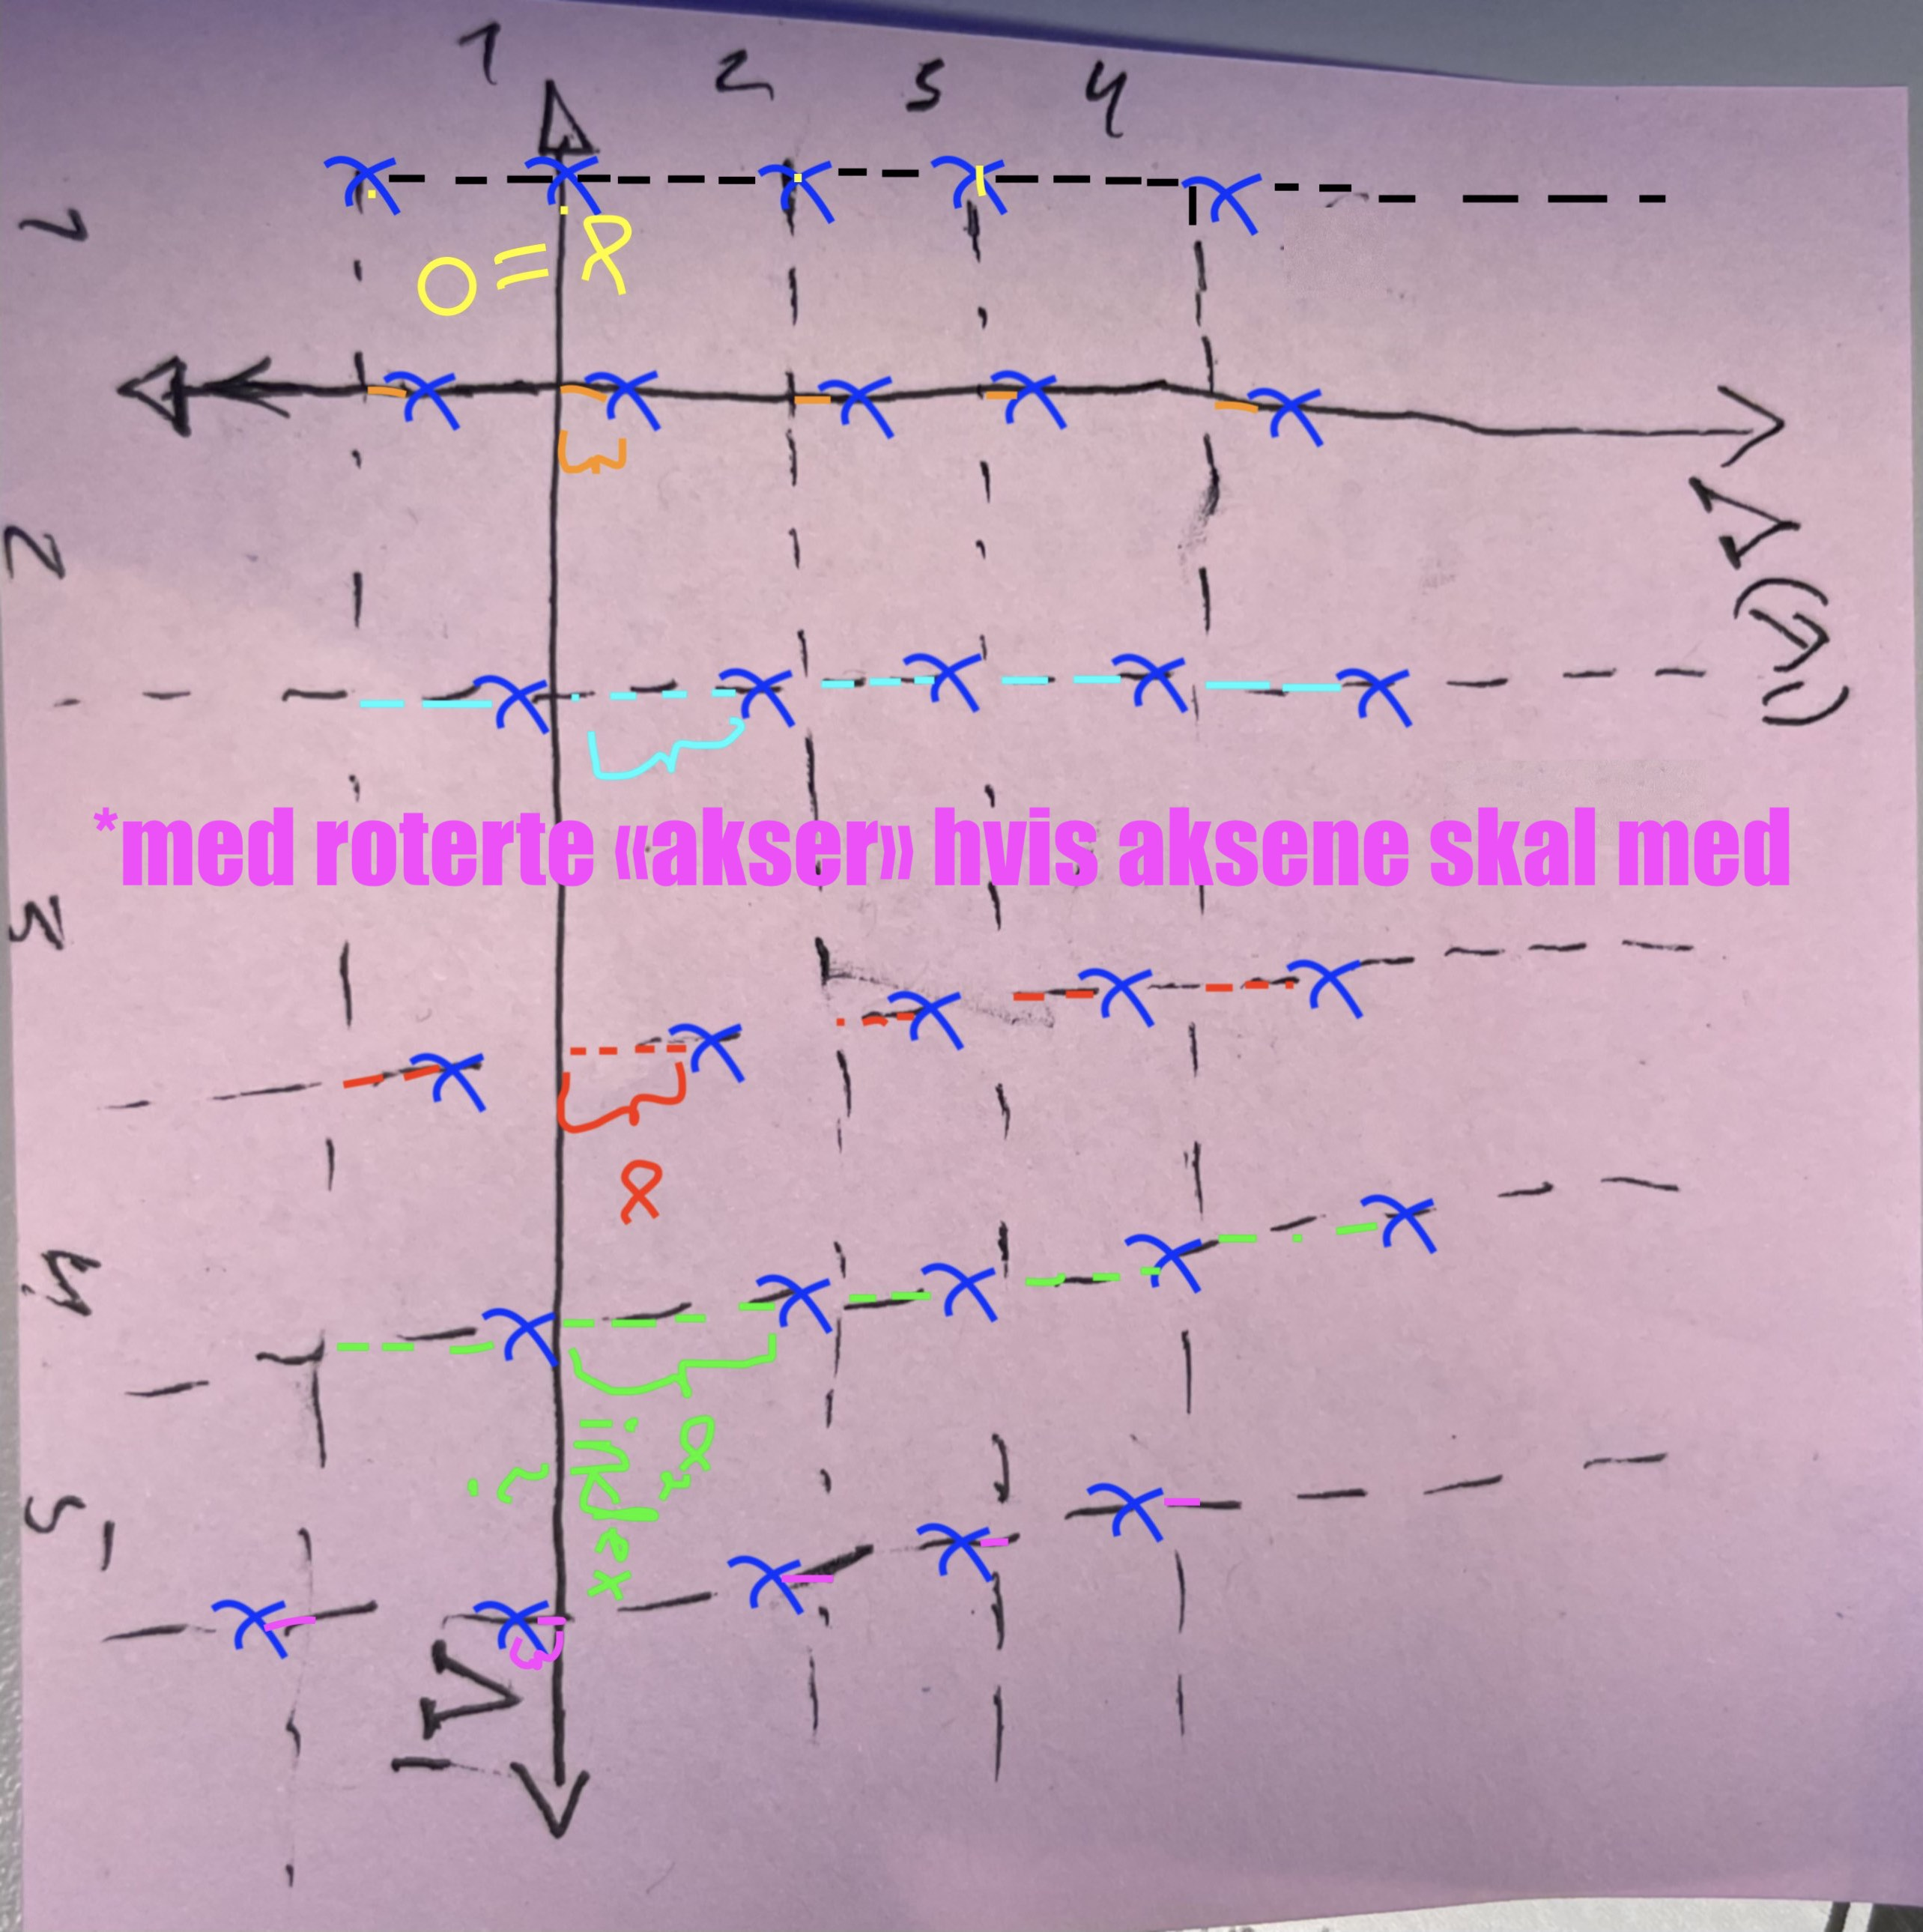
\includegraphics[width=0.9\linewidth]{multiple_shift_left_zero_horizontal.jpg}
        %* Figure 4
        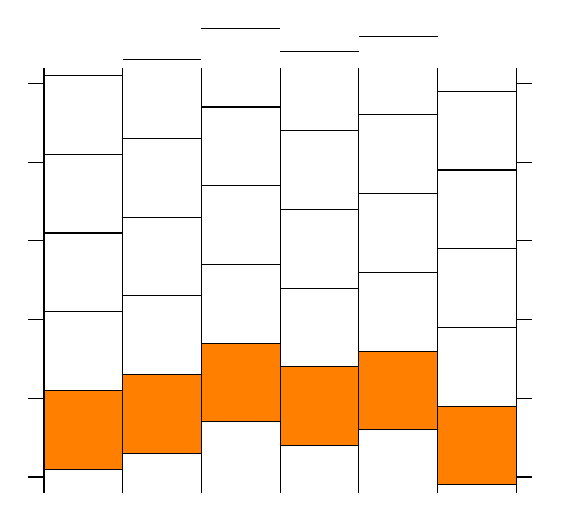
\begin{tikzpicture}[scale=1]
            % Define the tile
            \def\tile{
            % Draw the unit square
            \draw[fill=white] (0,0) rectangle (1,1);
            }
            \def\tiletwo{
            %\draw[fill=gray!65] (0,0) rectangle (1,1);
            \draw[fill=orange] (0,0) rectangle (1,1);
            %\draw[->] (0.5,0) -- (0.5,0.9);  % If arrows from the middle
            }

            % Shift list
            \def\BetaMinOne{0.1}
            \def\BetaZero{0.3}
            \def\BetaOne{0.7}
            \def\BetaTwo{0.4}
            \def\BetaThree{0.6}
            \def\BetaFour{-0.1}

            % Draw the tiling pattern
            \foreach \x in {0,1,2,3,4,5}{
                \foreach \y in {0,1,2,3}{
                    \ifnum\x=0
                        \pgfmathsetmacro{\shiftX}{\x}
                        \pgfmathsetmacro{\shiftY}{\y + \BetaMinOne}
                        \pgfmathsetmacro{\shiftSingle}{\BetaMinOne}
                    \fi
                    \ifnum\x=1
                        \pgfmathsetmacro{\shiftX}{\x}
                        \pgfmathsetmacro{\shiftY}{\y + \BetaZero}
                        \pgfmathsetmacro{\shiftSingle}{\BetaZero}
                    \fi
                    \ifnum\x=2
                        \pgfmathsetmacro{\shiftX}{\x} 
                        \pgfmathsetmacro{\shiftY}{\y + \BetaOne} 
                        \pgfmathsetmacro{\shiftSingle}{\BetaOne}
                    \fi
                    \ifnum\x=3
                        \pgfmathsetmacro{\shiftX}{\x}
                        \pgfmathsetmacro{\shiftY}{\y + \BetaTwo}
                        \pgfmathsetmacro{\shiftSingle}{\BetaTwo}
                    \fi
                    \ifnum\x=4
                        \pgfmathsetmacro{\shiftX}{\x}
                        \pgfmathsetmacro{\shiftY}{\y + \BetaThree}
                        \pgfmathsetmacro{\shiftSingle}{\BetaThree}
                    \fi
                    \ifnum\x=5
                        \pgfmathsetmacro{\shiftX}{\x}
                        \pgfmathsetmacro{\shiftY}{\y + \BetaFour}
                        \pgfmathsetmacro{\shiftSingle}{\BetaFour}
                    \fi
                    % Drawing the bottom half-cubes
                    \ifnum\y=0
                        \draw[white, fill=white](\x,\y-0.2) rectangle (\x+1,\y+\shiftSingle);
                    \fi
                    % Drawing the top half-cubes
                    \ifnum\y=3
                        \ifthenelse{\lengthtest{\shiftSingle pt > 0.2 pt}}{
                            \draw[white] (\x,\y+2+\shiftSingle) -- (\x+1,\y+2+\shiftSingle);  % Top
                        }{
                        \draw[black] (\x,\y+2+\shiftSingle) -- (\x+1,\y+2+\shiftSingle);  % Top
                        }
                        \draw[black] (\x,\y+1) -- (\x,\y+2);  % Left line
                        \draw[black] (\x+1,\y+2) -- (\x+1,\y+1);  % Right line
                        \draw[black] (\x+1,\y+1+\shiftSingle) -- (\x,\y+1+\shiftSingle);  % Bottom line
                        %\draw[red, fill=red](\x,\y+1) rectangle (\x+1,\y+2);
                    \fi
                    % Drawing the rest of the middle cubes
                    \begin{scope}[shift={(\shiftX,\shiftY)}]
                        \tile
                    \end{scope}
                    % Drawing a new line of shifted colored cubes on top at the first row
                    \ifnum\y=0
                        \begin{scope}[shift={(\shiftX,\shiftY)}]
                            \tiletwo
                        \end{scope}
                    \fi
                }  
            }
            % get the outline grid 
            % small black lines at the left and right
            \foreach \y in {0,1,2,3,4,5}{
                \draw (0-0.2,\y) -- (0,\y);  % Left
                \draw (6,\y) -- (6+0.2,\y);  % Right
            }
            % small black lines at the top and bottom
            \foreach \x in {0,1,2,3,4,5,6}{
                %\draw (\x,0-0.2) -- (\x,0);  % Top
                %\draw (\x,5) -- (\x,5+0.2);  % Bottom
                \draw (\x,0-0.2) -- (\x,5+0.2);  % Shift only in the vertical direction, therefore only one line
            }
        \end{tikzpicture}
        %* —————————————————
        \caption{Multiple column shifts}
        \label{fig:multiple_shift_vertical_tiling}
    \end{subfigure}
    \caption{Text}
    \label{fig:tiling_figures}
\end{figure}

\extractcolorspecs{Cyan}{\myColorModel}{\myColor} orange is \myColor\ in model %\myColorModel
